\documentclass[a4paper]{article}
% maxwidth is the original width if it is less than linewidth
% otherwise use linewidth (to make sure the graphics do not exceed the margin)
\makeatletter
\def\maxwidth{ %
  \ifdim\Gin@nat@width>\linewidth
    \linewidth
  \else
    \Gin@nat@width
  \fi
}
\makeatother

\usepackage[utf8]{inputenc}
\usepackage{a4wide,paralist}
\usepackage{amsmath, amssymb, xfrac, amsthm}
\usepackage{dsfont}
\usepackage{xcolor}
\usepackage{amsfonts}
\usepackage{graphicx}
\usepackage{hyperref}
\usepackage{bm}
\usepackage{underscore}

% for showing python code blocks
\usepackage{listings}
\lstdefinestyle{pythonstyle}{
    language=Python,
    backgroundcolor=\color[HTML]{F0F0F0},
    commentstyle=\color[HTML]{44515E},
    keywordstyle=\color[HTML]{228A96},
    numberstyle=\color[HTML]{F36E3A},
    stringstyle=\color[HTML]{6BA77F},
    basicstyle=\ttfamily\small,        
    breakatwhitespace=false,          
    breaklines=true,                  
    captionpos=b,                     
    keepspaces=true,                  
    numbers=none,                     
    numbersep=5pt,                   
    showspaces=false,                
    showstringspaces=false,
    showtabs=false,                  
    tabsize=4,
    literate=%
        {0}{{{\color[HTML]{F36E3A}0}}}1
        {1}{{{\color[HTML]{F36E3A}1}}}1
        {2}{{{\color[HTML]{F36E3A}2}}}1
        {3}{{{\color[HTML]{F36E3A}3}}}1
        {4}{{{\color[HTML]{F36E3A}4}}}1
        {5}{{{\color[HTML]{F36E3A}5}}}1
        {6}{{{\color[HTML]{F36E3A}6}}}1
        {7}{{{\color[HTML]{F36E3A}7}}}1
        {8}{{{\color[HTML]{F36E3A}8}}}1
        {9}{{{\color[HTML]{F36E3A}9}}}1
        {e+}{{{\color[HTML]{F36E3A}e+}}}1
        {e-}{{{\color[HTML]{F36E3A}e-}}}1,
}

\lstdefinestyle{rstyle}{
    language=R,
    backgroundcolor=\color[HTML]{F0F0F0},
    commentstyle=\color[HTML]{44515E},
    keywordstyle=\color[HTML]{228A96},
    numberstyle=\color[HTML]{F36E3A},
    stringstyle=\color[HTML]{6BA77F},
    basicstyle=\ttfamily\small,        
    breakatwhitespace=false,          
    breaklines=true,                  
    captionpos=b,                     
    keepspaces=true,                  
    numbers=none,                     
    numbersep=5pt,                   
    showspaces=false,                
    showstringspaces=false,
    showtabs=false,                  
    tabsize=4,
    literate=%
        {0}{{{\color[HTML]{F36E3A}0}}}1
        {1}{{{\color[HTML]{F36E3A}1}}}1
        {2}{{{\color[HTML]{F36E3A}2}}}1
        {3}{{{\color[HTML]{F36E3A}3}}}1
        {4}{{{\color[HTML]{F36E3A}4}}}1
        {5}{{{\color[HTML]{F36E3A}5}}}1
        {6}{{{\color[HTML]{F36E3A}6}}}1
        {7}{{{\color[HTML]{F36E3A}7}}}1
        {8}{{{\color[HTML]{F36E3A}8}}}1
        {9}{{{\color[HTML]{F36E3A}9}}}1
        {e+}{{{\color[HTML]{F36E3A}e+}}}1
        {e-}{{{\color[HTML]{F36E3A}e-}}}1,
    alsoletter ={_},
    otherkeywords = {!,!=,~,$,*,\&,\%/\%,\%*\%,\%\%,<-,<<-},
    morekeywords = {str_extract}
}

\lstset{style=pythonstyle}


% %exercise numbering
\renewcommand{\theenumi}{(\alph{enumi})}
\renewcommand{\theenumii}{\roman{enumii}}
\renewcommand\labelenumi{\theenumi}


\font \sfbold=cmssbx10

\setlength{\oddsidemargin}{0cm} \setlength{\textwidth}{16cm}


\sloppy
\parindent0em
\parskip0.5em
\topmargin-2.3 cm
\textheight25cm
\textwidth17.5cm
\oddsidemargin-0.8cm
\pagestyle{empty}


\newcommand{\kopfaml}[2]{
\hrule
\vspace{.15cm}
\begin{minipage}{\textwidth}
%akwardly i had to put \" here to make it compile correctly
	{\sf\bf Advanced Machine Learning \hfill Exercise sheet #1\\
	 \url{https://slds-lmu.github.io/i2ml/} \hfill #2}
\end{minipage}
\vspace{.05cm}
\hrule
\vspace{1cm}}


\newenvironment{allgemein}
	{\noindent}{\vspace{1cm}}

\newcounter{aufg}
\newenvironment{aufgabe}[1]
	{\refstepcounter{aufg}\textbf{Exercise \arabic{aufg}: #1}\\ \noindent}
	{\vspace{0.5cm}}

\newcounter{loes}
\newenvironment{loesung}[1]
	{\refstepcounter{loes}\textbf{Solution \arabic{loes}: #1}\\\noindent}
	{\bigskip}

\newenvironment{bonusaufgabe}
	{\refstepcounter{aufg}\textbf{Exercise \arabic{aufg}*\footnote{This
	is a bonus exercise.}:}\\ \noindent}
	{\vspace{0.5cm}}

\newenvironment{bonusloesung}
	{\refstepcounter{loes}\textbf{Solution \arabic{loes}*:}\\\noindent}
	{\bigskip}

\usepackage{caption}
\usepackage{subcaption}


\begin{document}

% dependencies: amsmath, amssymb, dsfont
% math spaces
\ifdefined\N
\renewcommand{\N}{\mathds{N}} % N, naturals
\else \newcommand{\N}{\mathds{N}} \fi
\newcommand{\Z}{\mathds{Z}} % Z, integers
\newcommand{\Q}{\mathds{Q}} % Q, rationals
\newcommand{\R}{\mathds{R}} % R, reals
\ifdefined\C
\renewcommand{\C}{\mathds{C}} % C, complex
\else \newcommand{\C}{\mathds{C}} \fi
\newcommand{\continuous}{\mathcal{C}} % C, space of continuous functions
\newcommand{\M}{\mathcal{M}} % machine numbers
\newcommand{\epsm}{\epsilon_m} % maximum error

% counting / finite sets
\newcommand{\setzo}{\{0, 1\}} % set 0, 1
\newcommand{\setmp}{\{-1, +1\}} % set -1, 1
\newcommand{\unitint}{[0, 1]} % unit interval

% basic math stuff
\newcommand{\xt}{\tilde x} % x tilde
\DeclareMathOperator*{\argmax}{arg\,max} % argmax
\DeclareMathOperator*{\argmin}{arg\,min} % argmin
\newcommand{\argminlim}{\mathop{\mathrm{arg\,min}}\limits} % argmax with limits
\newcommand{\argmaxlim}{\mathop{\mathrm{arg\,max}}\limits} % argmin with limits
\newcommand{\sign}{\operatorname{sign}} % sign, signum
\newcommand{\I}{\mathbb{I}} % I, indicator
\newcommand{\order}{\mathcal{O}} % O, order
\newcommand{\bigO}{\mathcal{O}} % Big-O Landau
\newcommand{\littleo}{{o}} % Little-o Landau
\newcommand{\pd}[2]{\frac{\partial{#1}}{\partial #2}} % partial derivative
\newcommand{\floorlr}[1]{\left\lfloor #1 \right\rfloor} % floor
\newcommand{\ceillr}[1]{\left\lceil #1 \right\rceil} % ceiling
\newcommand{\indep}{\perp \!\!\! \perp} % independence symbol

% sums and products
\newcommand{\sumin}{\sum\limits_{i=1}^n} % summation from i=1 to n
\newcommand{\sumim}{\sum\limits_{i=1}^m} % summation from i=1 to m
\newcommand{\sumjn}{\sum\limits_{j=1}^n} % summation from j=1 to p
\newcommand{\sumjp}{\sum\limits_{j=1}^p} % summation from j=1 to p
\newcommand{\sumik}{\sum\limits_{i=1}^k} % summation from i=1 to k
\newcommand{\sumkg}{\sum\limits_{k=1}^g} % summation from k=1 to g
\newcommand{\sumjg}{\sum\limits_{j=1}^g} % summation from j=1 to g
\newcommand{\meanin}{\frac{1}{n} \sum\limits_{i=1}^n} % mean from i=1 to n
\newcommand{\meanim}{\frac{1}{m} \sum\limits_{i=1}^m} % mean from i=1 to n
\newcommand{\meankg}{\frac{1}{g} \sum\limits_{k=1}^g} % mean from k=1 to g
\newcommand{\prodin}{\prod\limits_{i=1}^n} % product from i=1 to n
\newcommand{\prodkg}{\prod\limits_{k=1}^g} % product from k=1 to g
\newcommand{\prodjp}{\prod\limits_{j=1}^p} % product from j=1 to p

% linear algebra
\newcommand{\one}{\bm{1}} % 1, unitvector
\newcommand{\zero}{\mathbf{0}} % 0-vector
\newcommand{\id}{\bm{I}} % I, identity
\newcommand{\diag}{\operatorname{diag}} % diag, diagonal
\newcommand{\trace}{\operatorname{tr}} % tr, trace
\newcommand{\spn}{\operatorname{span}} % span
\newcommand{\scp}[2]{\left\langle #1, #2 \right\rangle} % <.,.>, scalarproduct
\newcommand{\mat}[1]{\begin{pmatrix} #1 \end{pmatrix}} % short pmatrix command
\newcommand{\Amat}{\mathbf{A}} % matrix A
\newcommand{\Deltab}{\mathbf{\Delta}} % error term for vectors

% basic probability + stats
\renewcommand{\P}{\mathds{P}} % P, probability
\newcommand{\E}{\mathds{E}} % E, expectation
\newcommand{\var}{\mathsf{Var}} % Var, variance
\newcommand{\cov}{\mathsf{Cov}} % Cov, covariance
\newcommand{\corr}{\mathsf{Corr}} % Corr, correlation
\newcommand{\normal}{\mathcal{N}} % N of the normal distribution
\newcommand{\iid}{\overset{i.i.d}{\sim}} % dist with i.i.d superscript
\newcommand{\distas}[1]{\overset{#1}{\sim}} % ... is distributed as ...

% machine learning
\newcommand{\Xspace}{\mathcal{X}} % X, input space
\newcommand{\Yspace}{\mathcal{Y}} % Y, output space
\newcommand{\Zspace}{\mathcal{Z}} % Space of sampled datapoints ! Also defined identically in ml-online.tex !
\newcommand{\nset}{\{1, \ldots, n\}} % set from 1 to n
\newcommand{\pset}{\{1, \ldots, p\}} % set from 1 to p
\newcommand{\gset}{\{1, \ldots, g\}} % set from 1 to g
\newcommand{\Pxy}{\mathbb{P}_{xy}} % P_xy
\newcommand{\Exy}{\mathbb{E}_{xy}} % E_xy: Expectation over random variables xy
\newcommand{\xv}{\mathbf{x}} % vector x (bold)
\newcommand{\xtil}{\tilde{\mathbf{x}}} % vector x-tilde (bold)
\newcommand{\yv}{\mathbf{y}} % vector y (bold)
\newcommand{\xy}{(\xv, y)} % observation (x, y)
\newcommand{\xvec}{\left(x_1, \ldots, x_p\right)^\top} % (x1, ..., xp)
\newcommand{\Xmat}{\mathbf{X}} % Design matrix
\newcommand{\allDatasets}{\mathds{D}} % The set of all datasets
\newcommand{\allDatasetsn}{\mathds{D}_n}  % The set of all datasets of size n
\newcommand{\D}{\mathcal{D}} % D, data
\newcommand{\Dn}{\D_n} % D_n, data of size n
\newcommand{\Dtrain}{\mathcal{D}_{\text{train}}} % D_train, training set
\newcommand{\Dtest}{\mathcal{D}_{\text{test}}} % D_test, test set
\newcommand{\xyi}[1][i]{\left(\xv^{(#1)}, y^{(#1)}\right)} % (x^i, y^i), i-th observation
\newcommand{\Dset}{\left( \xyi[1], \ldots, \xyi[n]\right)} % {(x1,y1)), ..., (xn,yn)}, data
\newcommand{\defAllDatasetsn}{(\Xspace \times \Yspace)^n} % Def. of the set of all datasets of size n
\newcommand{\defAllDatasets}{\bigcup_{n \in \N}(\Xspace \times \Yspace)^n} % Def. of the set of all datasets
\newcommand{\xdat}{\left\{ \xv^{(1)}, \ldots, \xv^{(n)}\right\}} % {x1, ..., xn}, input data
\newcommand{\ydat}{\left\{ \yv^{(1)}, \ldots, \yv^{(n)}\right\}} % {y1, ..., yn}, input data
\newcommand{\yvec}{\left(y^{(1)}, \hdots, y^{(n)}\right)^\top} % (y1, ..., yn), vector of outcomes
\renewcommand{\xi}[1][i]{\xv^{(#1)}} % x^i, i-th observed value of x
\newcommand{\yi}[1][i]{y^{(#1)}} % y^i, i-th observed value of y
\newcommand{\xivec}{\left(x^{(i)}_1, \ldots, x^{(i)}_p\right)^\top} % (x1^i, ..., xp^i), i-th observation vector
\newcommand{\xj}{\xv_j} % x_j, j-th feature
\newcommand{\xjvec}{\left(x^{(1)}_j, \ldots, x^{(n)}_j\right)^\top} % (x^1_j, ..., x^n_j), j-th feature vector
\newcommand{\phiv}{\mathbf{\phi}} % Basis transformation function phi
\newcommand{\phixi}{\mathbf{\phi}^{(i)}} % Basis transformation of xi: phi^i := phi(xi)

%%%%%% ml - models general
\newcommand{\lamv}{\bm{\lambda}} % lambda vector, hyperconfiguration vector
\newcommand{\Lam}{\bm{\Lambda}}	 % Lambda, space of all hpos
% Inducer / Inducing algorithm
\newcommand{\preimageInducer}{\left(\defAllDatasets\right)\times\Lam} % Set of all datasets times the hyperparameter space
\newcommand{\preimageInducerShort}{\allDatasets\times\Lam} % Set of all datasets times the hyperparameter space
% Inducer / Inducing algorithm
\newcommand{\ind}{\mathcal{I}} % Inducer, inducing algorithm, learning algorithm

% continuous prediction function f
\newcommand{\ftrue}{f_{\text{true}}}  % True underlying function (if a statistical model is assumed)
\newcommand{\ftruex}{\ftrue(\xv)} % True underlying function (if a statistical model is assumed)
\newcommand{\fx}{f(\xv)} % f(x), continuous prediction function
\newcommand{\fdomains}{f: \Xspace \rightarrow \R^g} % f with domain and co-domain
\newcommand{\Hspace}{\mathcal{H}} % hypothesis space where f is from
\newcommand{\fbayes}{f^{\ast}} % Bayes-optimal model
\newcommand{\fxbayes}{f^{\ast}(\xv)} % Bayes-optimal model
\newcommand{\fkx}[1][k]{f_{#1}(\xv)} % f_j(x), discriminant component function
\newcommand{\fh}{\hat{f}} % f hat, estimated prediction function
\newcommand{\fxh}{\fh(\xv)} % fhat(x)
\newcommand{\fxt}{f(\xv ~|~ \thetab)} % f(x | theta)
\newcommand{\fxi}{f\left(\xv^{(i)}\right)} % f(x^(i))
\newcommand{\fxih}{\hat{f}\left(\xv^{(i)}\right)} % f(x^(i))
\newcommand{\fxit}{f\left(\xv^{(i)} ~|~ \thetab\right)} % f(x^(i) | theta)
\newcommand{\fhD}{\fh_{\D}} % fhat_D, estimate of f based on D
\newcommand{\fhDtrain}{\fh_{\Dtrain}} % fhat_Dtrain, estimate of f based on D
\newcommand{\fhDnlam}{\fh_{\Dn, \lamv}} %model learned on Dn with hp lambda
\newcommand{\fhDlam}{\fh_{\D, \lamv}} %model learned on D with hp lambda
\newcommand{\fhDnlams}{\fh_{\Dn, \lamv^\ast}} %model learned on Dn with optimal hp lambda
\newcommand{\fhDlams}{\fh_{\D, \lamv^\ast}} %model learned on D with optimal hp lambda

% discrete prediction function h
\newcommand{\hx}{h(\xv)} % h(x), discrete prediction function
\newcommand{\hh}{\hat{h}} % h hat
\newcommand{\hxh}{\hat{h}(\xv)} % hhat(x)
\newcommand{\hxt}{h(\xv | \thetab)} % h(x | theta)
\newcommand{\hxi}{h\left(\xi\right)} % h(x^(i))
\newcommand{\hxit}{h\left(\xi ~|~ \thetab\right)} % h(x^(i) | theta)
\newcommand{\hbayes}{h^{\ast}} % Bayes-optimal classification model
\newcommand{\hxbayes}{h^{\ast}(\xv)} % Bayes-optimal classification model

% yhat
\newcommand{\yh}{\hat{y}} % yhat for prediction of target
\newcommand{\yih}{\hat{y}^{(i)}} % yhat^(i) for prediction of ith targiet
\newcommand{\resi}{\yi- \yih}

% theta
\newcommand{\thetah}{\hat{\theta}} % theta hat
\newcommand{\thetab}{\bm{\theta}} % theta vector
\newcommand{\thetabh}{\bm{\hat\theta}} % theta vector hat
\newcommand{\thetat}[1][t]{\thetab^{[#1]}} % theta^[t] in optimization
\newcommand{\thetatn}[1][t]{\thetab^{[#1 +1]}} % theta^[t+1] in optimization
\newcommand{\thetahDnlam}{\thetabh_{\Dn, \lamv}} %theta learned on Dn with hp lambda
\newcommand{\thetahDlam}{\thetabh_{\D, \lamv}} %theta learned on D with hp lambda
\newcommand{\mint}{\min_{\thetab \in \Theta}} % min problem theta
\newcommand{\argmint}{\argmin_{\thetab \in \Theta}} % argmin theta

% densities + probabilities
% pdf of x
\newcommand{\pdf}{p} % p
\newcommand{\pdfx}{p(\xv)} % p(x)
\newcommand{\pixt}{\pi(\xv~|~ \thetab)} % pi(x|theta), pdf of x given theta
\newcommand{\pixit}[1][i]{\pi\left(\xi[#1] ~|~ \thetab\right)} % pi(x^i|theta), pdf of x given theta
\newcommand{\pixii}[1][i]{\pi\left(\xi[#1]\right)} % pi(x^i), pdf of i-th x

% pdf of (x, y)
\newcommand{\pdfxy}{p(\xv,y)} % p(x, y)
\newcommand{\pdfxyt}{p(\xv, y ~|~ \thetab)} % p(x, y | theta)
\newcommand{\pdfxyit}{p\left(\xi, \yi ~|~ \thetab\right)} % p(x^(i), y^(i) | theta)

% pdf of x given y
\newcommand{\pdfxyk}[1][k]{p(\xv | y= #1)} % p(x | y = k)
\newcommand{\lpdfxyk}[1][k]{\log p(\xv | y= #1)} % log p(x | y = k)
\newcommand{\pdfxiyk}[1][k]{p\left(\xi | y= #1 \right)} % p(x^i | y = k)

% prior probabilities
\newcommand{\pik}[1][k]{\pi_{#1}} % pi_k, prior
\newcommand{\lpik}[1][k]{\log \pi_{#1}} % log pi_k, log of the prior
\newcommand{\pit}{\pi(\thetab)} % Prior probability of parameter theta

% posterior probabilities
\newcommand{\post}{\P(y = 1 ~|~ \xv)} % P(y = 1 | x), post. prob for y=1
\newcommand{\postk}[1][k]{\P(y = #1 ~|~ \xv)} % P(y = k | y), post. prob for y=k
\newcommand{\pidomains}{\pi: \Xspace \rightarrow \unitint} % pi with domain and co-domain
\newcommand{\pibayes}{\pi^{\ast}} % Bayes-optimal classification model
\newcommand{\pixbayes}{\pi^{\ast}(\xv)} % Bayes-optimal classification model
\newcommand{\pix}{\pi(\xv)} % pi(x), P(y = 1 | x)
\newcommand{\piv}{\bm{\pi}} % pi, bold, as vector
\newcommand{\pikx}[1][k]{\pi_{#1}(\xv)} % pi_k(x), P(y = k | x)
\newcommand{\pikxt}[1][k]{\pi_{#1}(\xv ~|~ \thetab)} % pi_k(x | theta), P(y = k | x, theta)
\newcommand{\pixh}{\hat \pi(\xv)} % pi(x) hat, P(y = 1 | x) hat
\newcommand{\pikxh}[1][k]{\hat \pi_{#1}(\xv)} % pi_k(x) hat, P(y = k | x) hat
\newcommand{\pixih}{\hat \pi(\xi)} % pi(x^(i)) with hat
\newcommand{\pikxih}[1][k]{\hat \pi_{#1}(\xi)} % pi_k(x^(i)) with hat
\newcommand{\pdfygxt}{p(y ~|~\xv, \thetab)} % p(y | x, theta)
\newcommand{\pdfyigxit}{p\left(\yi ~|~\xi, \thetab\right)} % p(y^i |x^i, theta)
\newcommand{\lpdfygxt}{\log \pdfygxt } % log p(y | x, theta)
\newcommand{\lpdfyigxit}{\log \pdfyigxit} % log p(y^i |x^i, theta)

% probababilistic
\newcommand{\bayesrulek}[1][k]{\frac{\P(\xv | y= #1) \P(y= #1)}{\P(\xv)}} % Bayes rule
\newcommand{\muk}{\bm{\mu_k}} % mean vector of class-k Gaussian (discr analysis)

% residual and margin
\newcommand{\eps}{\epsilon} % residual, stochastic
\newcommand{\epsi}{\epsilon^{(i)}} % epsilon^i, residual, stochastic
\newcommand{\epsh}{\hat{\epsilon}} % residual, estimated
\newcommand{\yf}{y \fx} % y f(x), margin
\newcommand{\yfi}{\yi \fxi} % y^i f(x^i), margin
\newcommand{\Sigmah}{\hat \Sigma} % estimated covariance matrix
\newcommand{\Sigmahj}{\hat \Sigma_j} % estimated covariance matrix for the j-th class

% ml - loss, risk, likelihood
\newcommand{\Lyf}{L\left(y, f\right)} % L(y, f), loss function
\newcommand{\Lypi}{L\left(y, \pi\right)} % L(y, pi), loss function
\newcommand{\Lxy}{L\left(y, \fx\right)} % L(y, f(x)), loss function
\newcommand{\Lxyi}{L\left(\yi, \fxi\right)} % loss of observation
\newcommand{\Lxyt}{L\left(y, \fxt\right)} % loss with f parameterized
\newcommand{\Lxyit}{L\left(\yi, \fxit\right)} % loss of observation with f parameterized
\newcommand{\Lxym}{L\left(\yi, f\left(\bm{\tilde{x}}^{(i)} ~|~ \thetab\right)\right)} % loss of observation with f parameterized
\newcommand{\Lpixy}{L\left(y, \pix\right)} % loss in classification
\newcommand{\Lpiv}{L\left(y, \piv\right)} % loss in classification
\newcommand{\Lpixyi}{L\left(\yi, \pixii\right)} % loss of observation in classification
\newcommand{\Lpixyt}{L\left(y, \pixt\right)} % loss with pi parameterized
\newcommand{\Lpixyit}{L\left(\yi, \pixit\right)} % loss of observation with pi parameterized
\newcommand{\Lhxy}{L\left(y, \hx\right)} % L(y, h(x)), loss function on discrete classes
\newcommand{\Lr}{L\left(r\right)} % L(r), loss defined on residual (reg) / margin (classif)
\newcommand{\lone}{|y - \fx|} % L1 loss
\newcommand{\ltwo}{\left(y - \fx\right)^2} % L2 loss
\newcommand{\lbernoullimp}{\ln(1 + \exp(-y \cdot \fx))} % Bernoulli loss for -1, +1 encoding
\newcommand{\lbernoullizo}{- y \cdot \fx + \log(1 + \exp(\fx))} % Bernoulli loss for 0, 1 encoding
\newcommand{\lcrossent}{- y \log \left(\pix\right) - (1 - y) \log \left(1 - \pix\right)} % cross-entropy loss
\newcommand{\lbrier}{\left(\pix - y \right)^2} % Brier score
\newcommand{\risk}{\mathcal{R}} % R, risk
\newcommand{\riskbayes}{\mathcal{R}^\ast}
\newcommand{\riskf}{\risk(f)} % R(f), risk
\newcommand{\riskdef}{\E_{y|\xv}\left(\Lxy \right)} % risk def (expected loss)
\newcommand{\riskt}{\mathcal{R}(\thetab)} % R(theta), risk
\newcommand{\riske}{\mathcal{R}_{\text{emp}}} % R_emp, empirical risk w/o factor 1 / n
\newcommand{\riskeb}{\bar{\mathcal{R}}_{\text{emp}}} % R_emp, empirical risk w/ factor 1 / n
\newcommand{\riskef}{\riske(f)} % R_emp(f)
\newcommand{\risket}{\mathcal{R}_{\text{emp}}(\thetab)} % R_emp(theta)
\newcommand{\riskr}{\mathcal{R}_{\text{reg}}} % R_reg, regularized risk
\newcommand{\riskrt}{\mathcal{R}_{\text{reg}}(\thetab)} % R_reg(theta)
\newcommand{\riskrf}{\riskr(f)} % R_reg(f)
\newcommand{\riskrth}{\hat{\mathcal{R}}_{\text{reg}}(\thetab)} % hat R_reg(theta)
\newcommand{\risketh}{\hat{\mathcal{R}}_{\text{emp}}(\thetab)} % hat R_emp(theta)
\newcommand{\LL}{\mathcal{L}} % L, likelihood
\newcommand{\LLt}{\mathcal{L}(\thetab)} % L(theta), likelihood
\newcommand{\LLtx}{\mathcal{L}(\thetab | \xv)} % L(theta|x), likelihood
\newcommand{\logl}{\ell} % l, log-likelihood
\newcommand{\loglt}{\logl(\thetab)} % l(theta), log-likelihood
\newcommand{\logltx}{\logl(\thetab | \xv)} % l(theta|x), log-likelihood
\newcommand{\errtrain}{\text{err}_{\text{train}}} % training error
\newcommand{\errtest}{\text{err}_{\text{test}}} % test error
\newcommand{\errexp}{\overline{\text{err}_{\text{test}}}} % avg training error

% lm
\newcommand{\thx}{\thetab^\top \xv} % linear model
\newcommand{\olsest}{(\Xmat^\top \Xmat)^{-1} \Xmat^\top \yv} % OLS estimator in LM


\kopfaml{10}{Imbalanced Learning}

\loesung{Cost Curves}{

\begin{enumerate}
    \item We can simply retrieve the FPRs and TPRs from the table (or matrix) and plot the curves.
\begin{lstlisting}
import numpy as np
import matplotlib.pyplot as plt

# The first column is FPR, the second column is TPR
FPR_TPR_1 = np.array(
    [[0.0, 0.00],
     [0.1, 0.60],
     [0.2, 0.75],
     [0.3, 0.825],
     [0.4, 0.85],
     [0.5, 0.875],
     [0.6, 0.90],
     [0.7, 0.925],
     [0.8, 0.950],
     [0.9, 0.975],
     [1.0, 1.0]])

FPR_TPR_2 = np.array(
    [[0.0, 0.00],
     [0.1, 0.2],
     [0.2, 0.4],
     [0.3, 0.6],
     [0.4, 0.8],
     [0.5, 0.925],
     [0.6, 0.96],
     [0.7, 0.98],
     [0.8, 0.99],
     [0.9, 0.995],
     [1.0, 1.00]]
)


def draw_roc_curves(fpr_tpr_1: np.ndarray, fpr_tpr_2: np.ndarray) -> None:
    fig, ax = plt.subplots(1, 1, figsize=(8, 7))
    ax.plot(fpr_tpr_1[:, 0], fpr_tpr_1[:, 1], marker='o', label='Classifier 1')
    ax.plot(fpr_tpr_2[:, 0], fpr_tpr_2[:, 1], marker='o', label='Classifier 2')

    ax.set_xlabel('False Positive Rate')
    ax.set_ylabel('True Positive Rate')
    ax.grid('on')

    plt.legend()
    plt.savefig('roc_curves.pdf', bbox_inches='tight')
\end{lstlisting}
The ROC curves are shown in Figure~\ref{fig:roc_curves}
\begin{figure}[h]
    \centering
    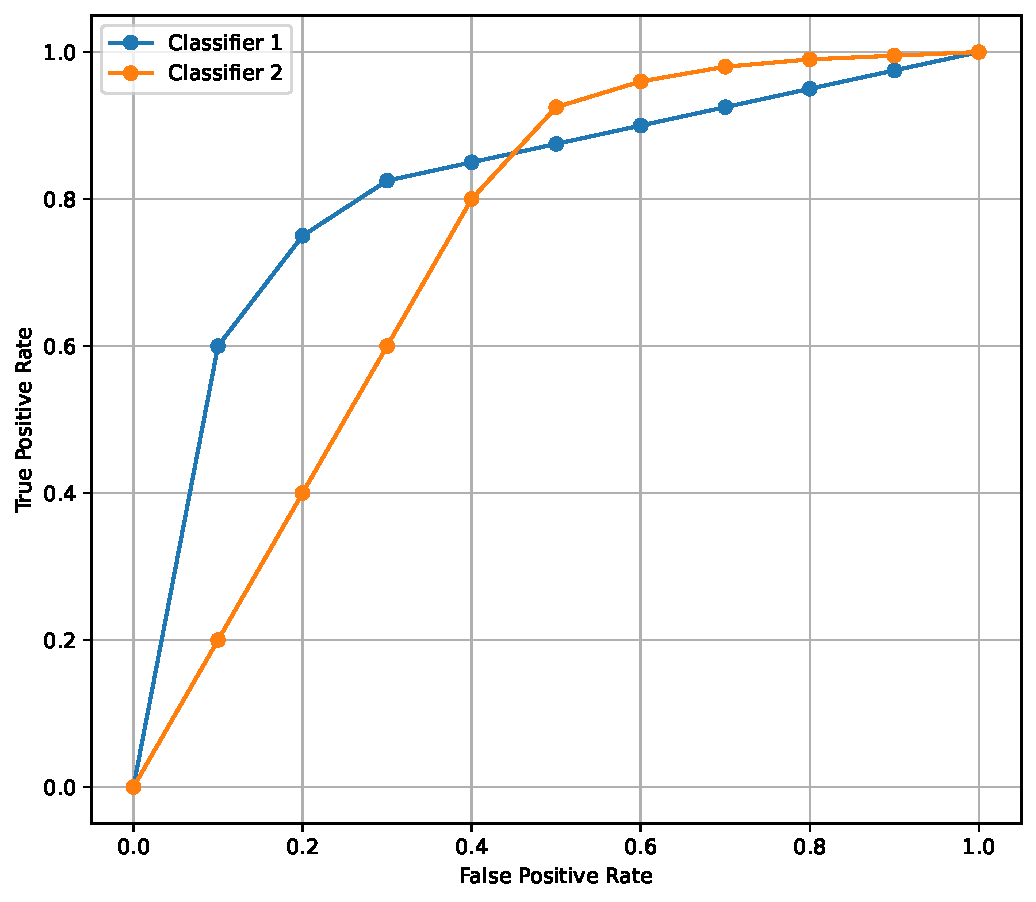
\includegraphics[width=0.5\textwidth]{figures/roc_curves}
    \caption{ROC Curves.}
    \label{fig:roc_curves}
\end{figure}

\item The cost is computed as 
\begin{align*}
    \rho_{MCE} = (FNR - FPR) \cdot \pi_{+} + FPR
\end{align*}
For each $(FPR, TPR)$ point in the ROC space, we draw a line of $(\pi_{+}, \rho_{MCE})$.

\begin{lstlisting}

def draw_cost_curves(fpr_tpr_1: np.ndarray, fpr_tpr_2: np.ndarray) -> None:
    fnr_1 = 1 - fpr_tpr_1[:, 1]
    fnr_2 = 1 - fpr_tpr_2[:, 1]
    # Probability of positive
    # Assume P = 50 points in [0.0, 1.0]
    pos_probs = np.linspace(0.0, 1.0, 50)

    # Compute the coefficient (FNR - FPR)
    # Shape after expansion: (N, 1), where N is the number of points in ROC space.
    fnr_minus_fpr_1 = np.expand_dims(fnr_1 - fpr_tpr_1[:, 0], 1)
    fnr_minus_fpr_2 = np.expand_dims(fnr_2 - fpr_tpr_2[:, 0], 1)

    # Costs shape: (N, P)
    costs_1 = fnr_minus_fpr_1 * np.expand_dims(pos_probs, 0) + np.expand_dims(fpr_tpr_1[:, 0], 1)
    costs_2 = fnr_minus_fpr_2 * np.expand_dims(pos_probs, 0) + np.expand_dims(fpr_tpr_2[:, 0], 1)
    # Point-wise minimum across cost lines.
    cost_curve_1 = costs_1.min(0)
    cost_curve_2 = costs_2.min(0)

    # Find the cross point of two cost curves. The following operation assumes that
    # cust_curve_1 is lower than cost_curve_2 in the beginning of the curves.
    cross_point_ind = np.flatnonzero(cost_curve_1 > cost_curve_2)[0]

    fig, ax = plt.subplots(1, 1, figsize=(8, 7))
    ax.plot(pos_probs, cost_curve_1, label='Classifier 1')
    ax.plot(pos_probs, cost_curve_2, label='Classifier_2')
    ax.vlines(
        pos_probs[cross_point_ind],
        ymin=0.0,
        ymax=cost_curve_1[cross_point_ind],
        linestyles='dashed',
        colors=['k'],
    )
    ax.set_xlabel('Probability of Positive')
    ax.set_ylabel('Error Rate')

    plt.legend()
    plt.savefig('cost_curves.pdf', bbox_inches='tight')


if __name__ == '__main__':
    draw_roc_curves(FPR_TPR_1, FPR_TPR_2)
    draw_cost_curves(FPR_TPR_1, FPR_TPR_2)

\end{lstlisting}
Then, we obtain Figure~\ref{fig:cost_curves}.

\begin{figure}[h]
    \centering
    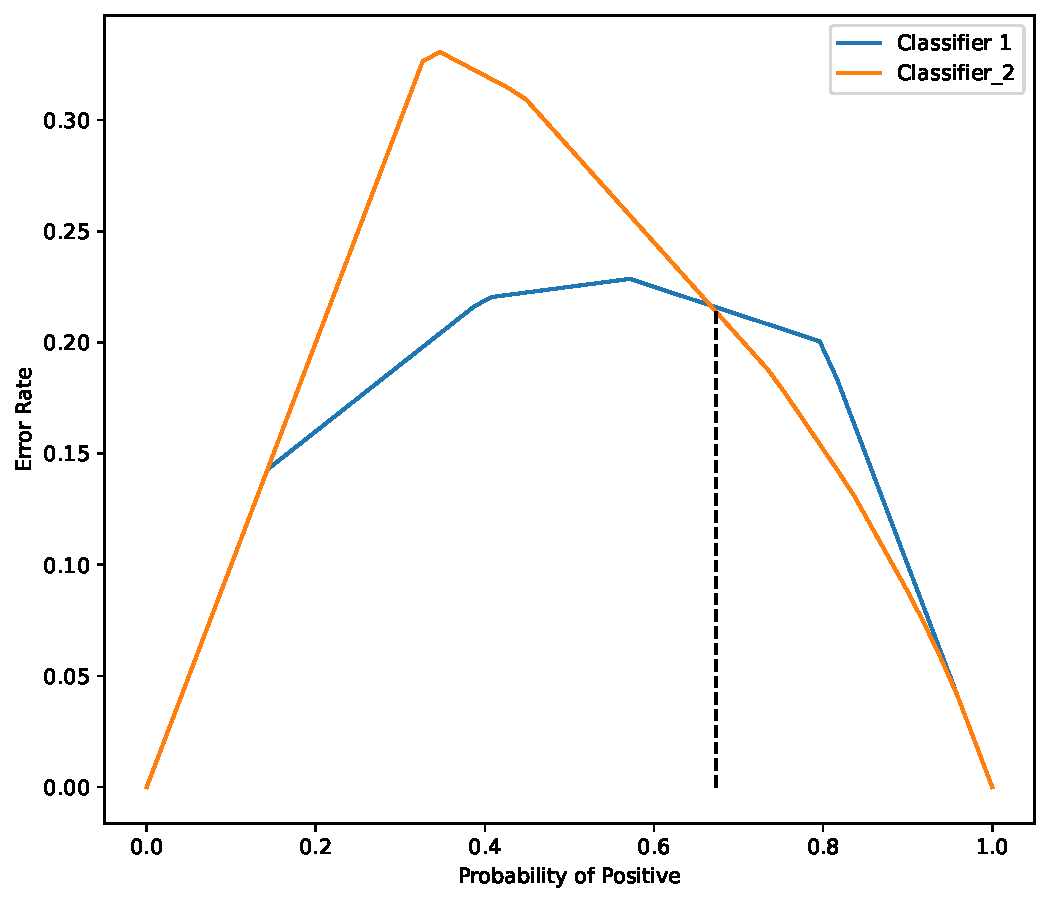
\includegraphics[width=0.5\textwidth]{figures/cost_curves}
    \caption{Cost Curves.}
    \label{fig:cost_curves}
\end{figure}

\end{enumerate}

}

\loesung{Tomek Links}{

\begin{enumerate}
\item 
\begin{lstlisting}

import matplotlib.pyplot as plt
import numpy as np

from sklearn.datasets import make_classification
from sklearn.metrics import pairwise_distances


def find_tomek_links(x: np.ndarray, y: np.ndarray) -> np.ndarray:
    """Find Tomek Links in samples.

    Args:
        x: Data samples with shape (num_samples, num_features).
        y: Binary class labels with shape (num_samples,). 
           1 means positive class, 0 means negative class.

    Returns:
        An array with shape (num_samples, ) with binary values, 
        for which 1 means that the corresponding sample 
        belongs to a Tomek link, while 0 means that the 
        sample does not belong to any Tomek link.
    """

    num_samples = x.shape[0]
    dist = pairwise_distances(x)

    # Compute the min. pairwise distance between samples with
    # pos. and neg. samples, respectively. To this end, we employ 
    # masked arrays, which can be constructed by
    # applying binary masks to the original array. In the masks, 1
    # means excluding the corresponding samples when performing 
    # operations e.g. min, argmin, etc.

    # pos_mask has shape (num_samples, num_samples).
    pos_mask = np.tile(np.expand_dims(1-y, 0), (num_samples, 1))
    # Also excluding each sample itself.
    # Otherwise, argmin will always point to the sample itself.
    pos_mask[np.arange(num_samples), np.arange(num_samples)] = True
    dist_pos = np.ma.array(dist, mask=pos_mask)
    # Sample indices indicate the closest positive sample to each data sample.
    min_dist_inds_pos = dist_pos.argmin(axis=1)

    neg_mask = np.tile(np.expand_dims(y, 0), (num_samples, 1))
    neg_mask[np.arange(num_samples), np.arange(num_samples)] = True
    dist_neg = np.ma.array(dist, mask=neg_mask)
    min_dist_inds_neg = dist_neg.argmin(axis=1)

    # This interpolation is equivalent to: if y_i = 1, then select the closest pos.
    # sample; if y_i = 0, then select the closest neg. sample. In other words, it
    # identifies the index of the closest intra-class sample.
    min_dist_inds_same_y = min_dist_inds_pos * y + min_dist_inds_neg * (1 - y)
    # This interpolation is equivalent to: if y_i = 1, then select the closest neg.
    # sample; if y_i = 0, then select the closest pos. sample. In other words, it
    # identifies the index of the closest inter-class sample.
    min_dist_inds_diff_y = min_dist_inds_pos * (1 - y) + min_dist_inds_neg * y
    # Retrieve the distance to the closest intra-class sample and 
    # inter-class sample
    min_dist_same_y = dist[np.arange(num_samples), min_dist_inds_same_y]
    min_dist_diff_y = dist[np.arange(num_samples), min_dist_inds_diff_y]

    # A sample belongs to a Tomek link if its closest inter-class sample is closer
    # than its closest intra-class sample.
    tomek_pairs = np.stack([np.arange(num_samples), min_dist_inds_diff_y], axis=1)
    # tomek_pairs has shape (num_tomek_pairs, 2) in the end
    tomek_pairs = tomek_pairs[min_dist_diff_y <= min_dist_same_y]

    # create a binary array and set the elements to 1 if the corresponding indices
    # appear in the tomek_pairs.
    is_tomek_sample = np.zeros((num_samples, ), dtype=bool)
    is_tomek_sample[tomek_pairs.flat] = True
    return is_tomek_sample

\end{lstlisting}

\item 

\begin{lstlisting}
def find_kept_samples(
        x: np.ndarray,
        y: np.ndarray,
        is_tomek_sample: np.ndarray
) -> np.ndarray:
    """Given the binary array indicating which sample belongs to a Tomek link. Find out which sample should be kept. The sample should be removed if it belongs to a Tomek link and it is majority class.

    Args:
        x: Data samples with shape (num_samples, num_features).
        y: Binary class labels with values 0 or 1.
        is_tomek_sample: A binary array with shape (num_samples,), 
            in which 1 means that the sample belongs to a Tomek link.

    Returns:
        A binary array with shape (num_samples,), in which 1 means that the 
        corresponding sample should be kept, otherwise it should be removed.
    """
    num_samples = x.shape[0]
    to_be_kept = np.ones((num_samples, ), dtype=bool)

    # Define which class is majority
    num_pos_samples = y.sum()
    num_neg_samples = num_samples - num_pos_samples
    if num_pos_samples >= num_neg_samples:
        y_major = 1
    else:
        y_major = 0

    # Only remove the sample in a Tomek link if it is majority class
    is_major_tomek_sample = np.logical_and(is_tomek_sample, y == y_major)
    to_be_kept[is_major_tomek_sample] = False

    return to_be_kept
\end{lstlisting}

\item 
\begin{lstlisting}
def run_experiment() -> None:
    # Generate data
    random_state = np.random.RandomState(11)
    x, y = make_classification(
        100,
        n_features=2,
        n_redundant=0,
        n_clusters_per_class=1,
        flip_y=0.02,
        class_sep=1.0,
        weights=[0.25, 0.75],
        random_state=random_state)

    # Plot the original dataset
    fig, ax = plt.subplots(1, 1)
    x_pos = x[y == 1]
    x_neg = x[y == 0]
    ax.scatter(x_pos[:, 0], x_pos[:, 1], facecolors='none', edgecolors='r', label='Pos. samples')
    ax.scatter(x_neg[:, 0], x_neg[:, 1], facecolors='none', edgecolors='b', label='Neg. samples')
    ax.set_title('Original Dataset')
    ax.set_xlim(-3, 3)
    ax.set_ylim(-3, 3)
    plt.legend()
    plt.savefig('original_dataset.pdf', bbox_inches='tight')
    plt.clf()

    # Find out which samples belong to Tomek links.
    is_tomek_link = find_tomek_links(x, y)

    fig, ax = plt.subplots(1, 1)
    x_tomek = x[is_tomek_link]
    ax.scatter(x_pos[:, 0], x_pos[:, 1], facecolors='none', edgecolors='r', label='Pos. samples')
    ax.scatter(x_neg[:, 0], x_neg[:, 1], facecolors='none', edgecolors='b', label='Neg. samples')
    ax.scatter(
        x_tomek[:, 0],
        x_tomek[:, 1],
        facecolors='none',
        edgecolors='g',
        label='Set of Tomek-link samples')
    ax.set_title('Set of Tomek-link samples')
    ax.set_xlim(-3, 3)
    ax.set_ylim(-3, 3)
    plt.legend()
    plt.savefig('tomek_links.pdf', bbox_inches='tight')
    plt.clf()

    # Identify which samples should be kept and which should be removed
    to_be_kept = find_kept_samples(x, y, is_tomek_link)

    fig, ax = plt.subplots(1, 1)
    x_removed = x[~to_be_kept]
    x, y = x[to_be_kept], y[to_be_kept]
    x_pos, x_neg = x[y == 1], x[y == 0]
    ax.scatter(x_pos[:, 0], x_pos[:, 1], facecolors='none', edgecolors='r', label='Pos. samples')
    ax.scatter(x_neg[:, 0], x_neg[:, 1], facecolors='none', edgecolors='b', label='Neg. samples')
    ax.scatter(
        x_removed[:, 0],
        x_removed[:, 1],
        facecolors='none',
        edgecolor='k',
        linestyle='dotted',
        label='Removed samples')
    ax.set_title('Majority Samples in Tomek links Removed')
    ax.set_xlim(-3, 3)
    ax.set_ylim(-3, 3)
    plt.legend()
    plt.savefig('subsampled_dataset.pdf', bbox_inches='tight')
    plt.clf()


if __name__ == '__main__':
    run_experiment()
\end{lstlisting}

After running the script, we obain the following figures:
\begin{figure}[h]
    \centering
    \begin{subfigure}{0.32\textwidth}
        \centering
        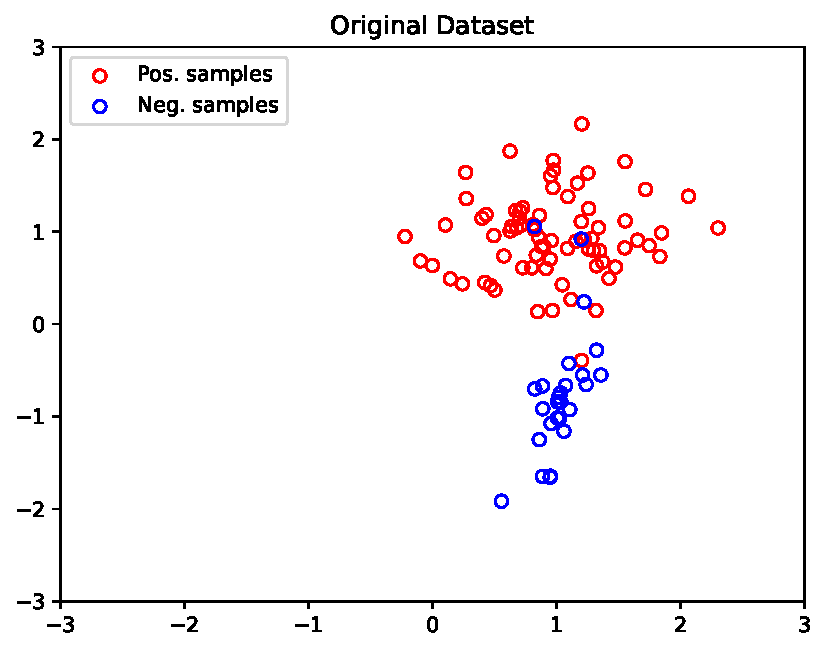
\includegraphics[width=\textwidth]{figures/original_dataset}
        \caption{Original Dataset.}
    \end{subfigure}
    \hfill
    \begin{subfigure}{0.32\textwidth}
        \centering
        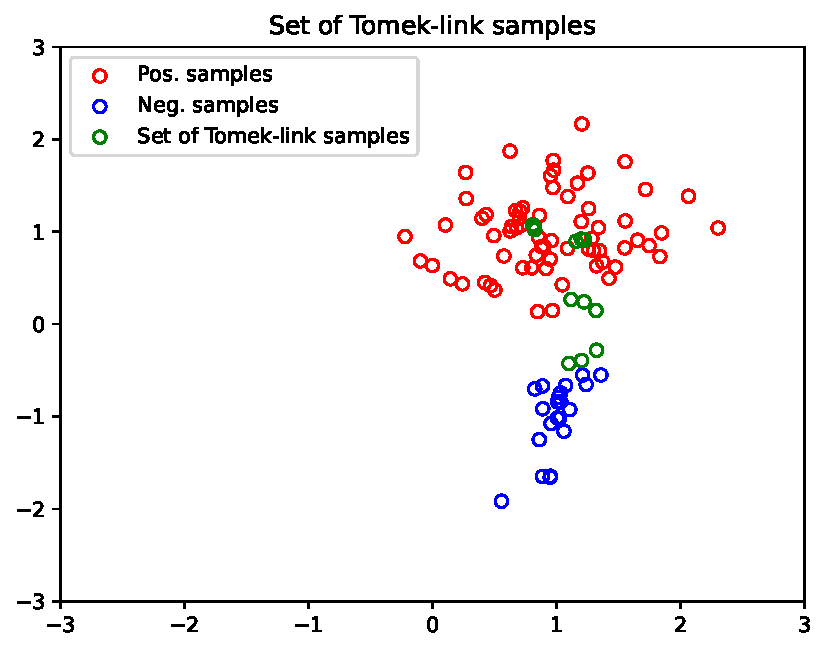
\includegraphics[width=\textwidth]{figures/tomek_links}
        \caption{Tomek Links.}
    \end{subfigure}
    \hfill
    \begin{subfigure}{0.32\textwidth}
        \centering
        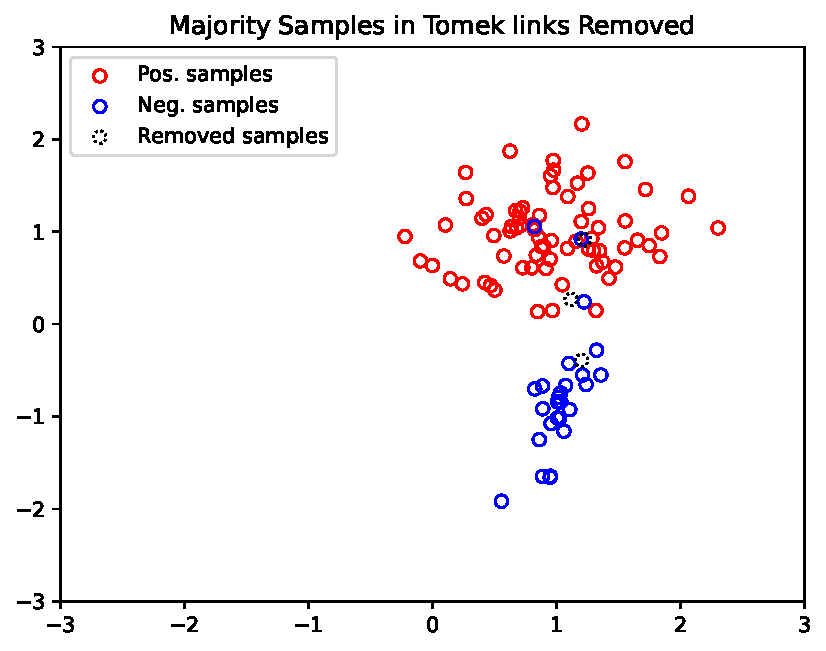
\includegraphics[width=\textwidth]{figures/removed_dataset}
        \caption{Subsampled Dataset.}
    \end{subfigure}
\end{figure}

\end{enumerate}


}






\end{document}
